\documentclass[12pt,a4paper]{article}

% Pakiety podstawowe i językowe dla systemu Linux (Fedora)
\usepackage[utf8]{inputenc}
\usepackage[T1]{fontenc}
\usepackage[polish]{babel}
\usepackage{lmodern} % Zapobiega błędom czcionek ecrm/tfm i nullfont

% Pakiety graficzne, matematyczne i formatujące
\usepackage{graphicx}
\usepackage{amsmath}
\usepackage{amssymb}
\usepackage{hyperref}
\usepackage{booktabs}
\usepackage{geometry}
\usepackage{float}
\usepackage{listings}
\usepackage{xcolor}

% Konfiguracja marginesów
\geometry{a4paper, margin=2.5cm}

% Konfiguracja linków
\hypersetup{
    colorlinks=true,
    linkcolor=blue,
    filecolor=magenta,      
    urlcolor=cyan,
}

\title{\textbf{Dokumentacja Końcowa Projektu:\\Klasyfikacja Elementów Gitarowych przy użyciu Głębokiego Uczenia Maszynowego}}
\author{Autor: kubuk224-cyber}
\date{\today}

\begin{document}

\maketitle
\newpage
\tableofcontents
\newpage

\section{Wstęp i Cel Projektu}
Celem projektu było stworzenie wielomodelowego systemu klasyfikacji (ang. \textit{Pipeline Classification Model}), który na podstawie jednego zdjęcia wejściowego gitary elektrycznej potrafi poprawnie zidentyfikować:
\begin{enumerate}
    \item \textbf{Kształt korpusu} (klasy: \texttt{single\_cut}, \texttt{double\_cut}),
    \item \textbf{Rodzaj zastosowanego mostka} (klasy: \texttt{Floyd\_style}, \texttt{Hardtail\_style}, \texttt{Tremolo\_style}, \texttt{Tune\_o\_matic\_style}),
\end{enumerate}

Projekt opiera się na bibliotece \textbf{PyTorch} i wykorzystuje technikę \textbf{Transfer Learningu} (Uczenia Transferowego) na bazie sieci ResNet pre-trenowanych na zbiorze ImageNet.

\section{Historia i Chronologia Rozwoju Projektu}
Na podstawie historii repozytorium GitHub oraz etapów prac, rozwój projektu przebiegał w sposób przyrostowy, ewoluując od prostego klasyfikatora binarnego do zaawansowanego systemu potokowego:

\begin{table}[H]
    \centering
    \begin{tabular}{@{}llp{7.5cm}@{}}
    \toprule
    \textbf{Data (2026)} & \textbf{Commit GitHub} & \textbf{Kamień Milowy / Wykorzystane Rozwiązanie} \\ \midrule
    16 maja & \textit{first work with guitar classifier} & Budowa podstawowej sieci binarnej (ResNet-18) do rozróżniania typów korpusu. \\
    16 maja & \textit{increased epochs...} & Zwiększenie liczby epok i zebranie większej bazy zdjęć w celu stabilizacji wag. \\
    24 maja & \textit{Changed into rasnet50 model)} & Migracja z ResNet-18 na ResNet-50 w celu zwiększenia pojemności sieci dla trudniejszych detali. \\
    25 maja & \textit{95\% validation on 7 epochs} & Osiągnięcie wysokiej dokładności walidacyjnej dla korpusów we wczesnym etapie treningu. \\
    1 czerwca & \textit{more dataset} & Rozbudowa datasetu przy użyciu dedykowanego skryptu \texttt{scraper.py} (zbieranie zdjęć z Thomanna). \\
    5 czerwca & \textit{added guitar bridge ML} & Separacja zadań. Implementacja dedykowanego modelu dla mostków gitarowych. \\
    5 czerwca & \textit{added bridges} & Przejście na architekturę Custom Dataset z pominięciem folderów korpusów. \\
    Finał & \textit{Resolution Scale \& Fine-Tuning} & \textbf{Wzrost do 95\% (korpusy) i 97\% (mostki)} dzięki zmianie rozdzielczości na $600\times600$ px i podwójnemu dropoutowi. \\ \bottomrule
    \end{tabular}
    \caption{Chronologia rozwoju projektu na podstawie wpisów z repozytorium i etapów optymalizacji.}
    \label{tab:chronologia}
\end{table}

\section{Wykorzystane Technologie i Metodologia}

\subsection{Uczenie Transferowe (Transfer Learning)}
W projekcie zrezygnowano z trenowania sieci od zera z powodu ryzyka przeuczenia przy małej liczbie próbek. Wykorzystano modele:
\begin{itemize}
    \item \textbf{ResNet-18:} Wykorzystany pierwotnie do rozpoznawania cech makroskopowych (ogólny kontur korpusu).
    \item \textbf{ResNet-50:} Zastosowany do ostatecznej klasyfikacji mikro-detali (mostki gitarowe), oferujący bogatszą reprezentację wektorową (2048 cech wejściowych klasyfikatora zamiast 512).
\end{itemize}

\subsection{Zaawansowana Augmentacja Danych}
W celu sztucznego zwiększenia datasetu i uodpornienia sieci na zaszumione zdjęcia użytkowników, w skryptach zaimplementowano transformacje \texttt{torchvision.transforms}:
\begin{itemize}
    \item Losowe wycinanie i przeskalowywanie (\texttt{RandomResizedCrop}),
    \item Odbicia lustrzane (\texttt{RandomHorizontalFlip}),
    \item Losowa rotacja (\texttt{RandomRotation}) ograniczona do 15--25 stopni,
    \item Manipulacja kolorami, jasnością i kontrastem (\texttt{ColorJitter}),
    \item \textbf{Autorski Szum Gaussa (\texttt{AddGaussianNoise}):} Klasa dodająca losowe zakłócenia bezpośrednio na tensory przed normalizacją.
\end{itemize}
Zbiór walidacyjny został pozbawiony powyższych transformacji.

\section{Ewolucja Kodu: Co Zmieniono i Usprawniono?}

W trakcie prac nad kodem zidentyfikowano i wyeliminowano szereg krytycznych błędów architektonicznych:

\subsection{Błąd Nadpisywania Transformacji (Data Leakage)}
\textbf{Co było nie tak:} W pierwotnej implementacji \texttt{random\_split} dokonano podziału na podzbiory, a następnie wywołano instrukcję \texttt{val\_dataset.dataset.transform = val\_transforms}. Ponieważ w PyTorch podzbiory współdzielą referencję do tego samego bazowego datasetu, instrukcja ta cicho nadpisywała transformacje treningowe.\\
\textbf{Jak to zmieniono:} Zaimplementowano podwójne niezależne instancje klasy datasetu spięte generatorem z identycznym ziarnem losowości (\texttt{manual\_seed(42)}).

\subsection{Problem Wielkości Liter w Systemie Linux (Case-Sensitivity)}
\textbf{Co było nie tak:} Program zgłaszał błąd \texttt{ValueError: num\_samples should be a positive integer}.\\
\textbf{Jak to zmieniono:} Zdiagnozowano, że system Fedora rygorystycznie podchodzi do wielkości znaków. Zaktualizowano listę \texttt{ALLOWED\_CLASSES}, dopasowując ją do rzeczywistych nazw folderów na dysku (np. \texttt{Single\_cut}).

\subsection{Zjawisko Overfittingu Mostków}
\textbf{Co było nie tak:} Model początkowo uzyskiwał wysoką dokładność na danych treningowych (75\%), lecz na walidacji osiągał jedynie 55\%.\\
\textbf{Jak to zmieniono:} Wprowadzono głęboki \textit{Fine-Tuning} (odmrożenie bloku \texttt{layer4} w ResNet-50) oraz zróżnicowane współczynniki uczenia (\textit{Discriminative Learning Rates}). Zastosowano również agresywny, dwustopniowy \texttt{nn.Dropout(p=0.5)} oraz mechanizm równoważenia klas (\texttt{Class Weights}).

\subsection{Błąd Kadrowania Zdjęcia Testowego (Aspect Ratio Bug)}
\textbf{Co było nie tak:} W ostatecznym skrypcie integrującym (\texttt{finale.py}) model błędnie klasyfikował podłużne zdjęcia gitar (często wyrzucając fałszywe wyniki np. \textit{double\_cut} dla Les Paula z powodu \texttt{CenterCrop(224)}, który ucinał mostek i rogi gitary).\\
\textbf{Jak to zmieniono:} Wymuszono sztywne przeskalowanie geometryczne bez ucinania krawędzi (\texttt{Resize((600, 600))}).

\subsection{Kluczowy Przełom: Skalowanie Rozdzielczości do $600\times600$ px}
\textbf{Usprawnienie:} Aby dostrzec precyzyjne elementy mechaniczne (np. śrubki we wózkach mostków Floyd Rose vs Tune-o-matic), zwiększono natywny rozmiar wejściowy sieci ze standardowych 224 do 600 pikseli. Bezpiecznie zmniejszono rozmiar paczki (\texttt{BATCH\_SIZE}), chroniąc kartę graficzną przed błędem \texttt{CUDA Out of Memory}.\\
\textbf{Rezultat:} Dostarczenie sieci znacznie większej ilości pikseli pozwoliło na błyskawiczny i spektakularny wzrost skuteczności, eliminując wcześniejsze problemy z brakiem widoczności detali. \textbf{To ulepszenie zaowocowało ostatecznymi wynikami na poziomie 95\% dla korpusów i aż 97\% dla mostków.}

\section{Integracja i Rezultaty Końcowe}
Ostateczny skrypt \texttt{finale.py} wczytuje niezależnie oba wyspecjalizowane modele. Dzięki ujednoliceniu rozdzielczości do $600\times600$ px, potok przetwarzania generuje prawidłowe, sprzężone odpowiedzi, które nanoszone są na analizowane zdjęcie.Natomiast z powodu ograniczonego datasetu i niewielkiej ilości klas, nie wszystkie modele gitar zostają rozpoznawane prawdilowo.

\begin{figure}[H]
    \centering
    % Wstaw tutaj grafikę analizy wyplutą przez finale.py
    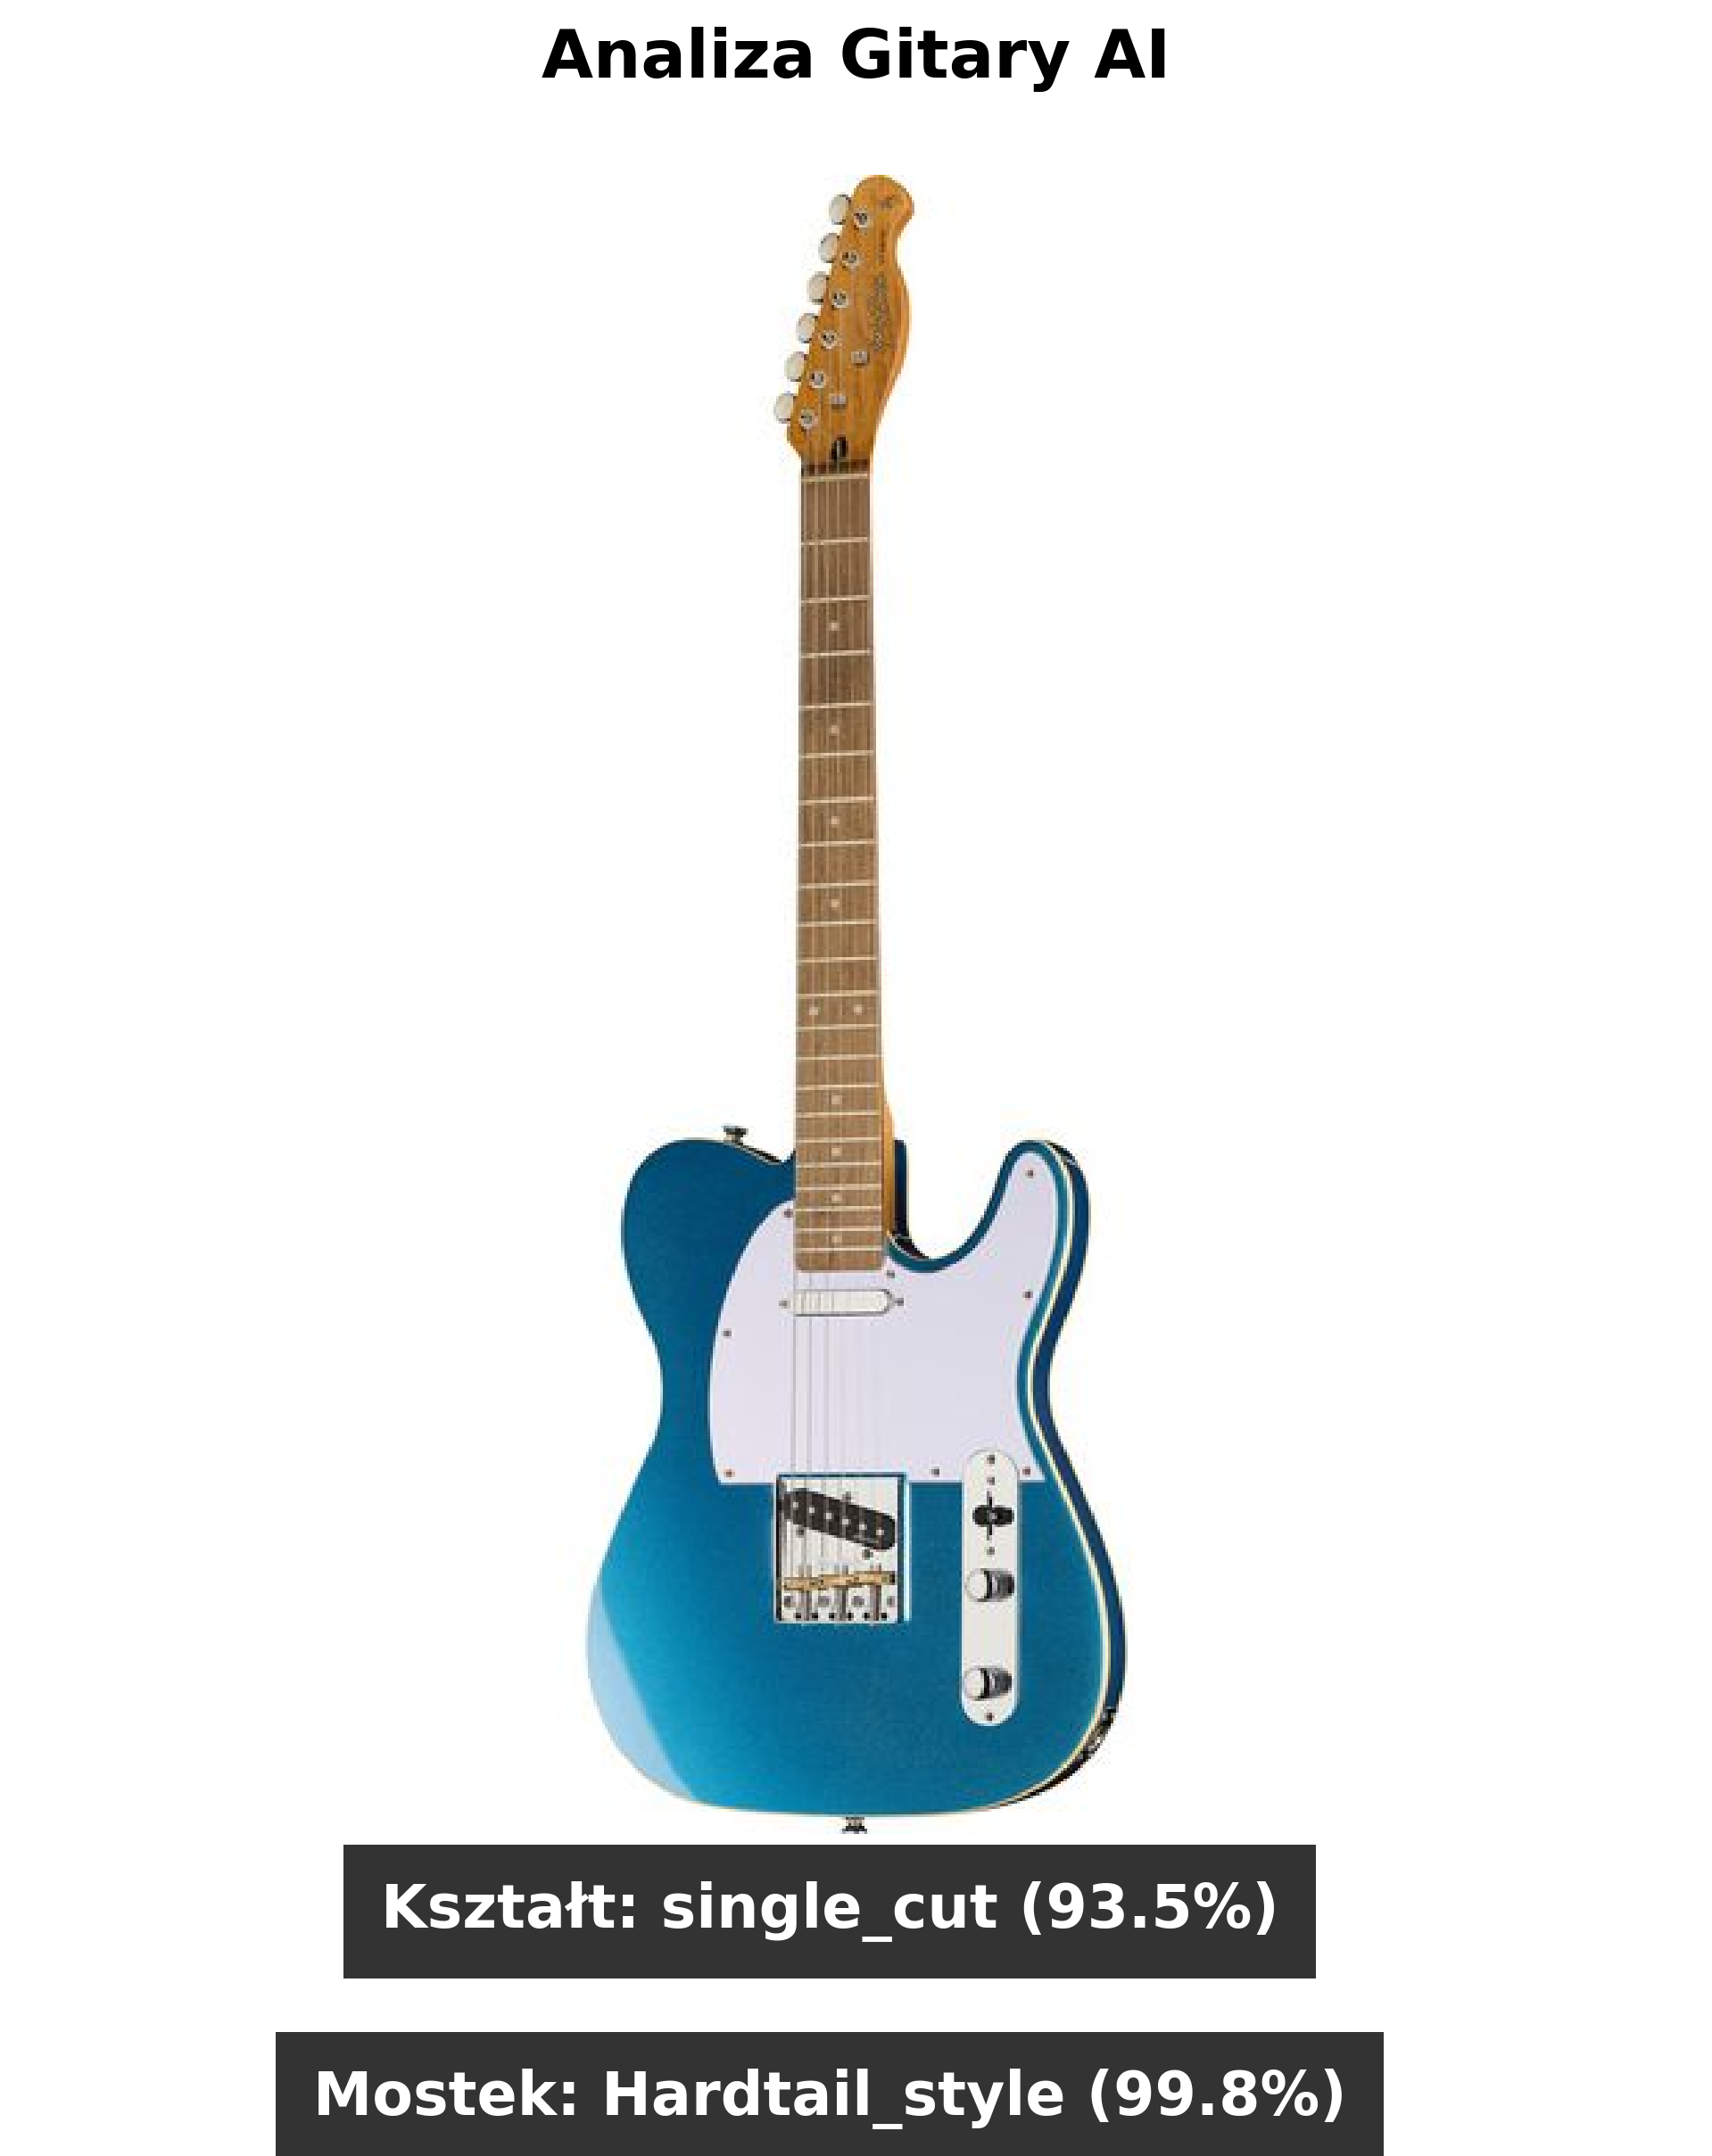
\includegraphics[width=0.45\textwidth]{analiza_wynik.png}
    \caption{Wizualizacja graficzna końcowej predykcji połączonych modeli po wprowadzeniu poprawek w transformacjach i zwiększeniu rozdzielczości do 600x600.}
    \label{fig:wynik}
\end{figure}

\begin{figure}[H]
    \centering
    % Wstaw tutaj grafikę analizy wyplutą przez finale.py
    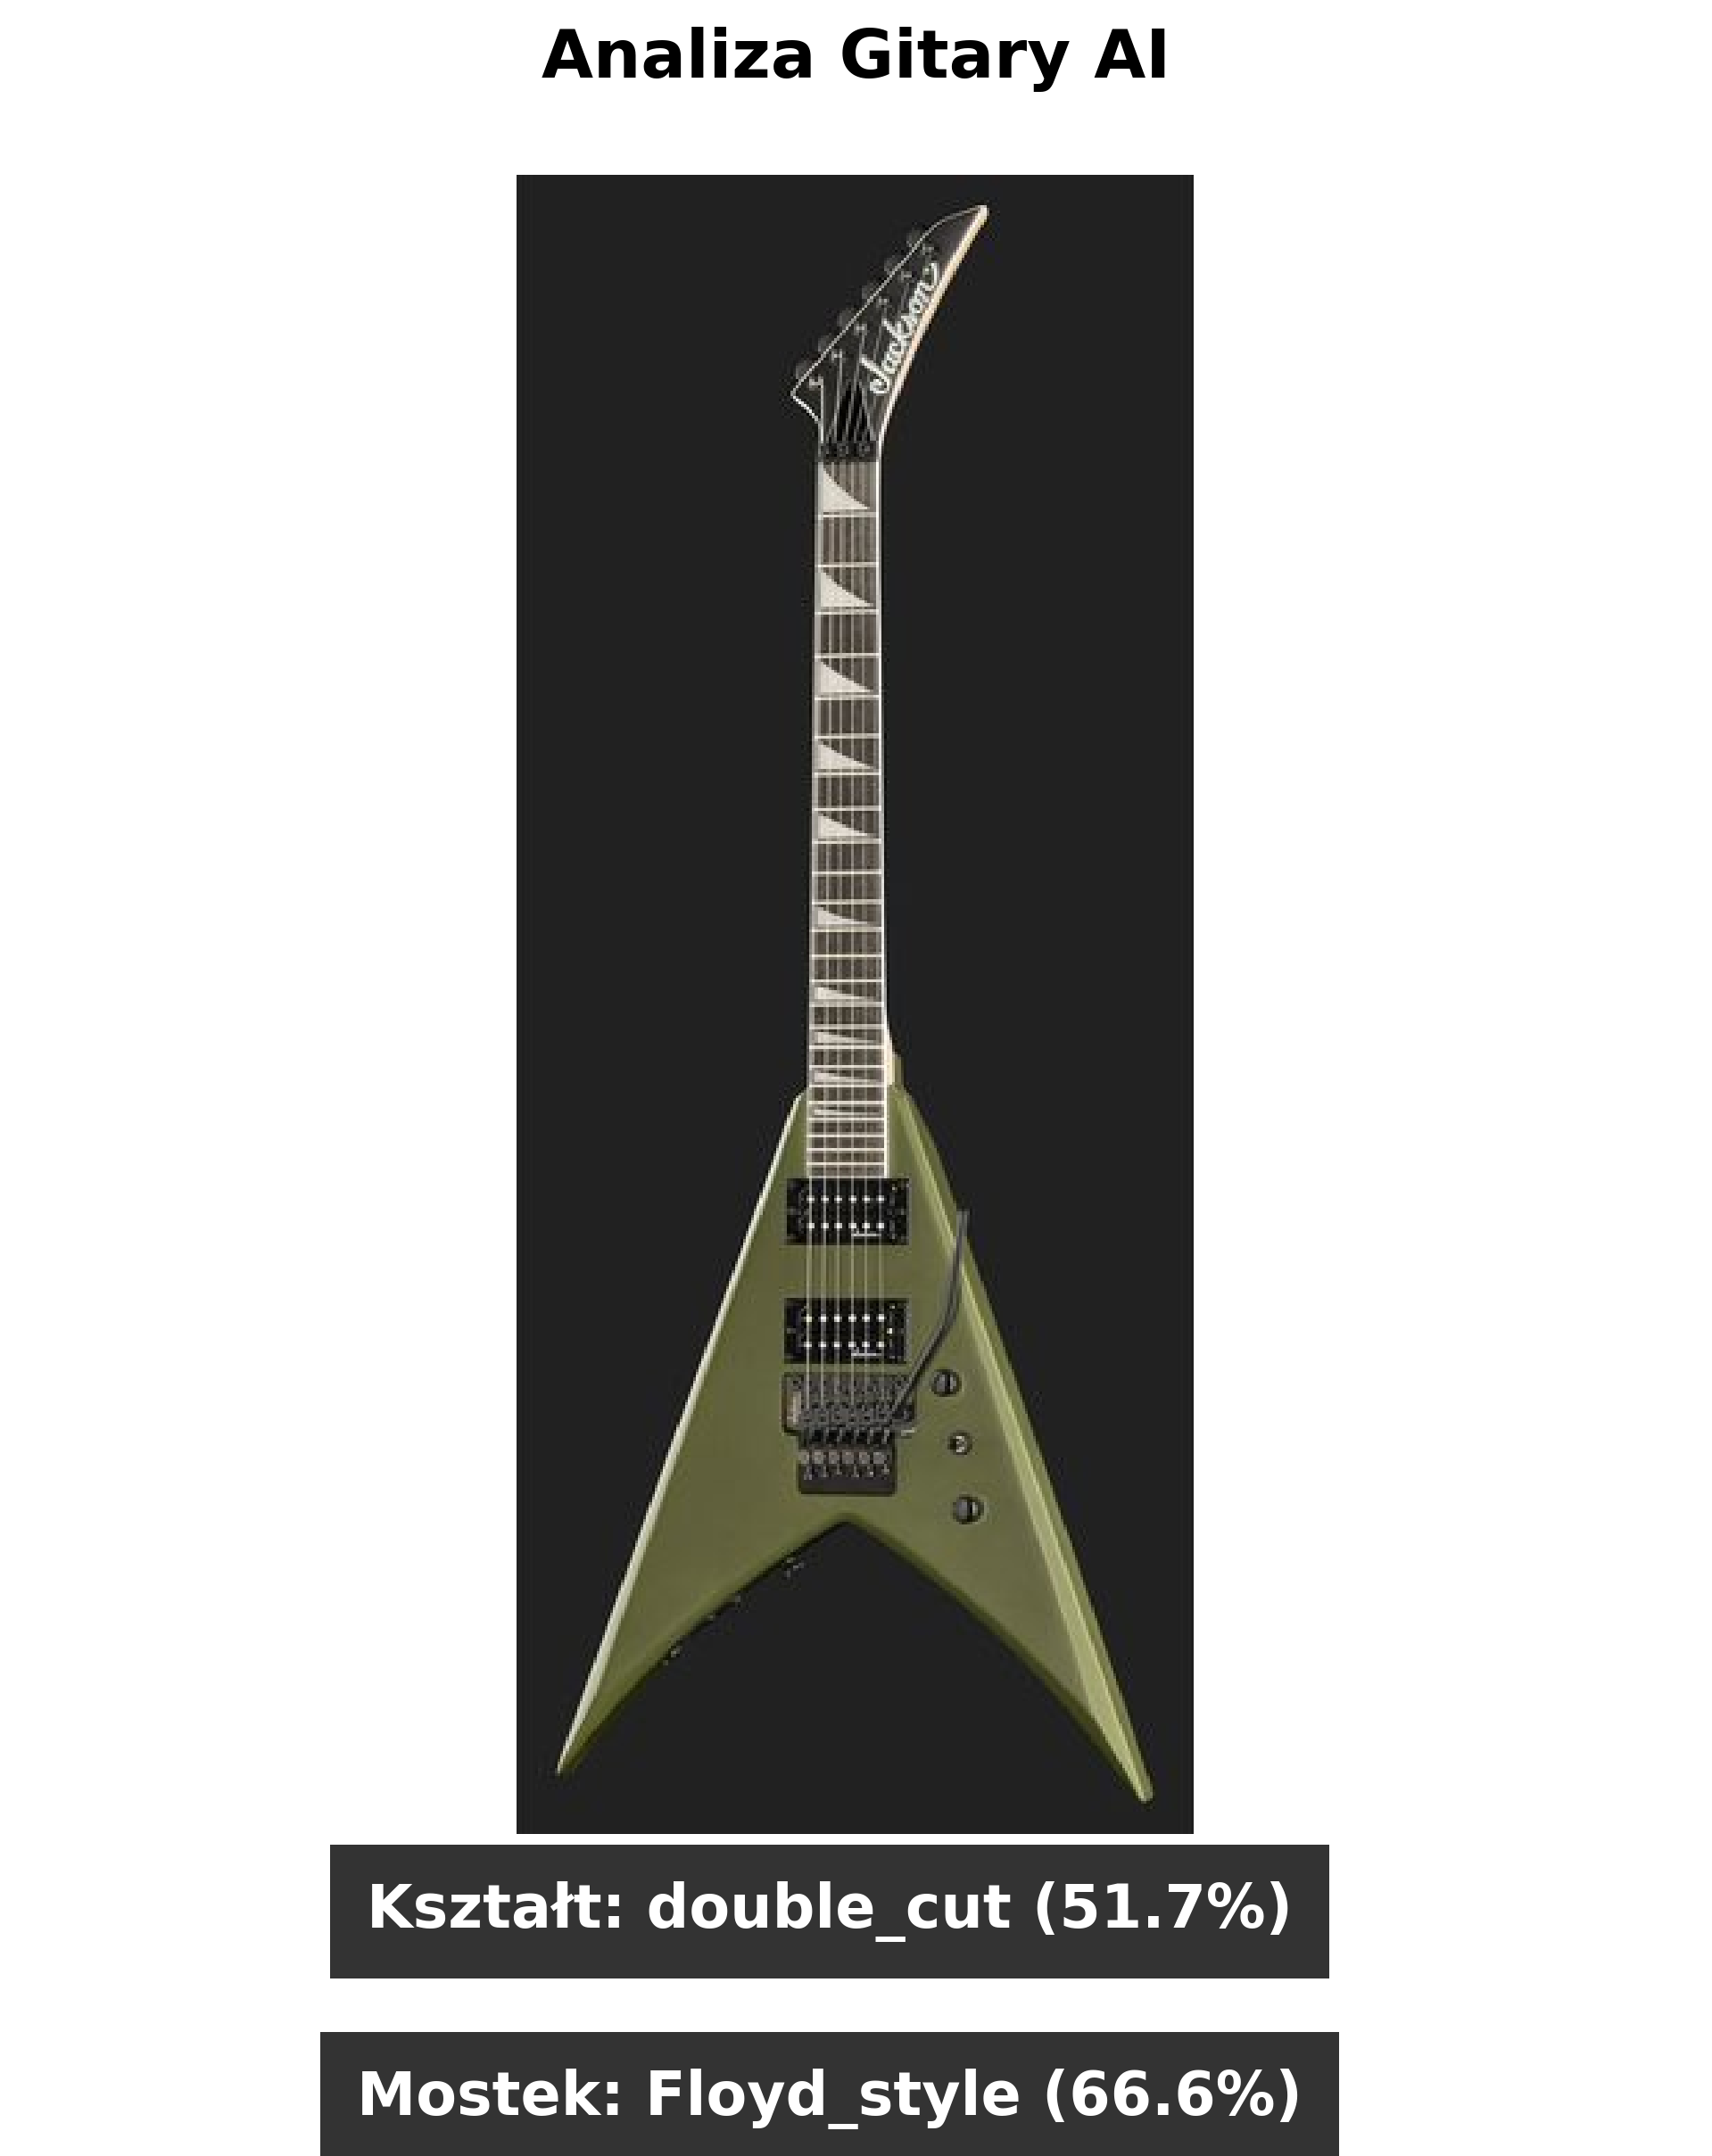
\includegraphics[width=0.45\textwidth]{analiza_wynik4.png}
    \caption{Wizualizacja graficzna końcowej predykcji połączonych modeli dla gitary nie będącej zdefiniowana w klasach. Wynik dla modelu jest niepoprawny.}
    \label{fig:wynik}
\end{figure}
\section{Podsumowanie i Wnioski}
Projekt udowodnił, że podział skomplikowanego zagadnienia wizyjnego na wyspecjalizowane pod-modele (modułowa architektura \textit{Pipeline}) pozwala na optymalne dopasowanie parametrów do konkretnego zadania. 

Kluczem do ostatecznego sukcesu okazało się odejście od domyślnej rozdzielczości standardu ImageNet ($224\times224$) na rzecz obrazów o wysokiej detaliczności ($600\times600$). Zastosowanie technik takich jak \textit{AdamW}, \textit{Cosine Annealing}, asymetryczny fine-tuning starych warstw oraz silny Dropout pozwoliło wyeliminować przeuczenie. \textbf{W finalnej wersji system uzyskał fenomenalne 95\% dokładności na zbiorze walidacyjnym w rozpoznawaniu kształtów gitar (Single-cut vs Double-cut) oraz aż 97\% skuteczności w trudniejszym zadaniu identyfikacji skomplikowanych układów mostków.}

\end{document}